\section{Overlay Accelerator Framework}
A block diagram of the proposed overlay accelerator system, based on an array of linear TM overlays~\cite{li2018time}, which supports both Zynq-based SoC and standalone PCIe accelerators, is shown in Figure~\ref{system}. 
The FPGA memory subsystem provides the interface between the overlay on the FPGA fabric and the ARM processor on a Zynq SoC via the AXI bus (or directly to the memory via the PCIe link). 
For the AXI bus-based overlay, two 32-bit FIFOs are used to connect a single 32-bit linear TM overlay with the memory subsystem. 
%For the PCIe-based overlay, four 32-bit linear TM overlays are used to make full use of the 128-bit data bandwidth and thus reduce the II to a quarter of that of a single overlay. 
For the PCIe-based overlay, we propose replicating four 32-bit linear TM overlays to make full use of the 128-bit data bandwidth. The four overlay instances can implement multiple compute kernels at runtime and thus reduce the II to a quarter of that of a single overlay. 
Data transfers between the internal memory subsystem, the DDR SDRAM and the offchip DRAM are under the control of a scatter-gather DMA engine. 
%The overlays are connected to the memory subsystem via two 128-bit FIFOs. 

\begin{figure}[tb]
	\centering
	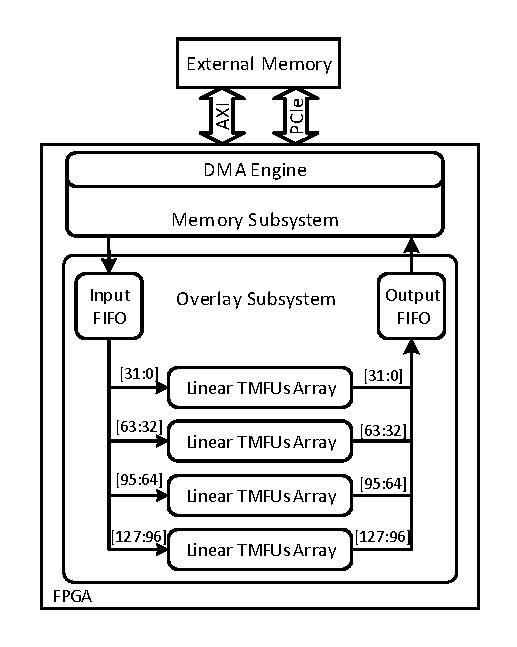
\includegraphics[width=\columnwidth]{Figures/system_new.pdf}
	\caption{The proposed overlay accelerator system.}
	\label{system}
\end{figure}

%\begin{figure}
%	\centering
%	\subfigure[Block diagram of the system]{
%	\centering
%	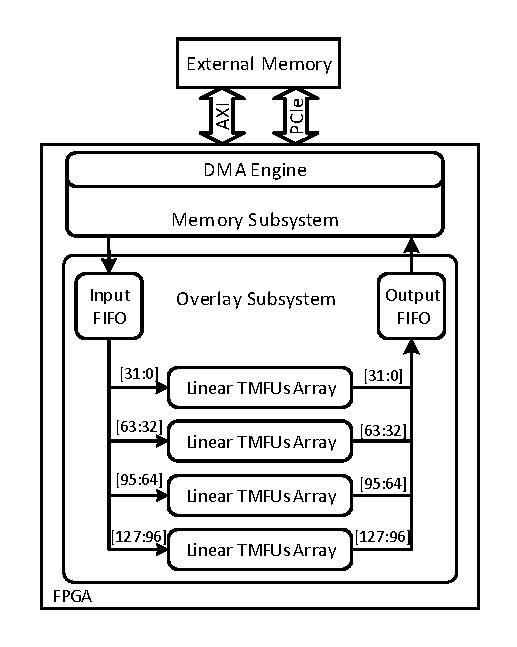
\includegraphics[width=0.9\columnwidth]{Figures/system_new.pdf}
%	\label{a}
%	}
%	~
%	\subfigure[A linear TM overlay]{
%	\centering
%	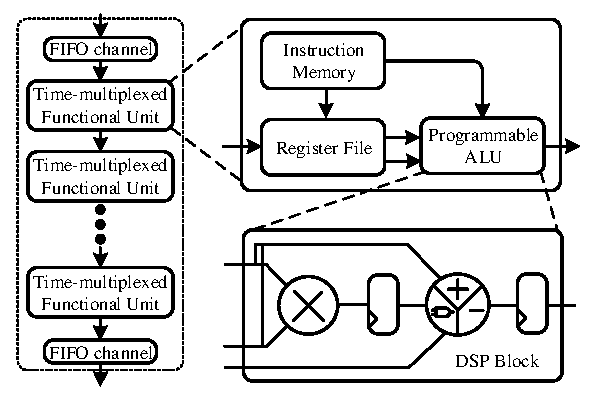
\includegraphics[width=0.9\columnwidth]{Figures/overlay.pdf}
%	\label{b}
%	}
%	\caption{The proposed overlay accelerator system.}
%	\label{system} %% label for entire figure
%\end{figure}


\subsection{Xillybus-Overlay}
Xillybus is a portable, easy to use DMA-based data transfer solution which provides a simple abstraction of the AXI/PCIe interfaces. 
%There is no prerequisite for knowledge of the AXI or PCIe protocols as all the low-level design is packaged into an IP core. 
One side of the Xillybus IP core is connected to the host processor, while the other side communicates with one standard FIFO, providing six signals to control the data flow. 
%, as shown in Figure~\ref{xillybus}. 
The host processor can be either the ARM processor of the Xilinx Zynq SoC (AXI-Xillybus: for an AXI bus-based solution) or a PC based x86 CPU (PCIe-Xillybus: for a PCIe-based solution). 
Xillybus provides a simple data loopback demo design, along with its driver for the default device files and the software code for testing purpose. 
%After the driver installation and the FPGA is programmed by the Xillybus bitstream, several device files are generated by the host driver which can be read from and written to like any file using basic Linux commands such as \textit{write} and \textit{read}. 
%Users have access to customize the Xillybus IP core by changing the number of device files, their streaming directions and data widths. 
When connecting Xillybus to the linear TM overlay, two standard FIFOs need be used to buffer the input/output data. 


%\begin{figure}[tb]
%	\centering
%	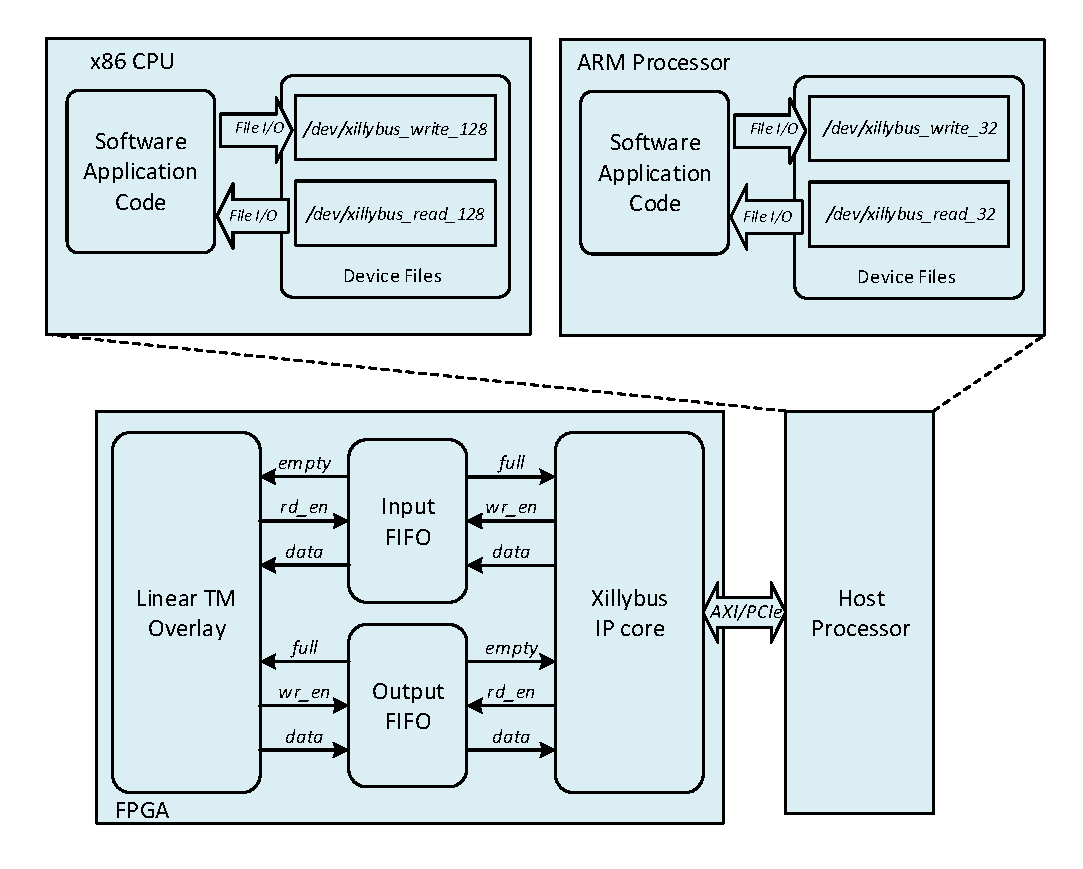
\includegraphics[width=0.9\columnwidth]{Figures/xillybus.pdf}
%	\caption{Xillybus-based overlay accelerator.}
%	\label{xillybus} 
%\end{figure}


\subsection{RIFFA-Overlay}
RIFFA has a more complicated framework which generally consists of three layers. 
%, as shown in Figure~\ref{riffa}. 
%It can be visually divided into two part, one part containing the device driver and the software APIs in the PC while the other one including all the PCIe hardware interface design in the FPGA. 
%A vendor-specific PCIe endpoint bridges the connection between RIFFA and host CPU via the PCIe link. 
%It is mainly comprised of three layers. 
On the bottom layer, an RX engine and a TX engine are connected to the vendor-specific PCIe Endpoint IP core, which bridges the connection between RIFFA and the host CPU. 
The middle layer supports up to 12 channels which send packets to the TX engine and receive packets from the RX engine through a scatter-gather DMA engine. 
The overlay which connects to the RX/TX FIFOs from the communication channels, is located on the top layer. 
An example design of one channel for data transfer, along with driver and software code, is provided. 
%Dedicated software APIs (\textit{fpga\_send} and \textit{fpga\_recv}) were developed as blocking functions.
Integration of the linear TM overlay with RIFFA is quite similar to that of Xillybus, except
that the standard FIFOs are replaced with first word fall through (FWFT) FIFOs to meet the timing closure. 
%For a more complicated design, multiple channels (up to 12 per FPGA) can be instantiated to integrate with different user cores independently. 

%\begin{figure}[tb]
%	\centering
%	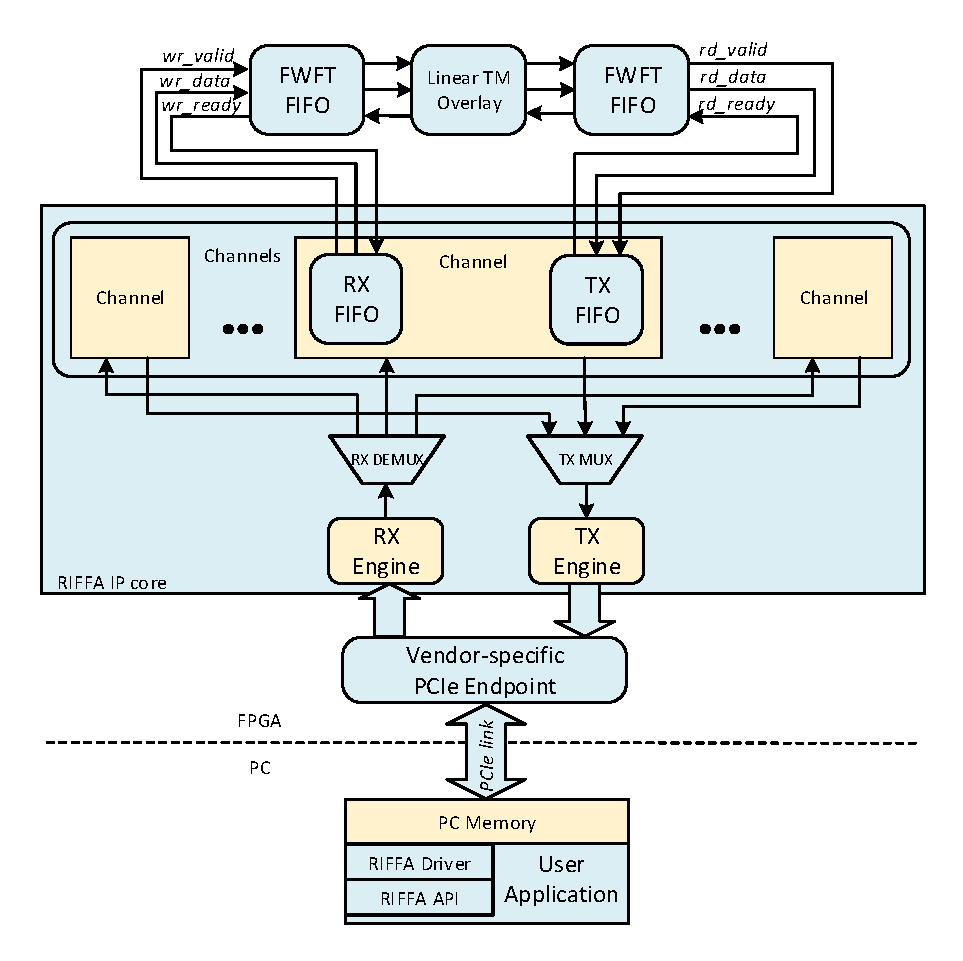
\includegraphics[width=0.9\columnwidth]{Figures/riffa.pdf}
%	\caption{RIFFA-based overlay accelerator.}
%	\label{riffa}
%\end{figure}


\subsection{DyRACT-Overlay}
The original version of DyRACT communication infrastructure enables PCIe-based high-speed communication between a host computer and FPGA-based user logic with support for partial reconfiguration (PR). 
It provisions multiple AXI4-stream backend interface, enabling seamless integration with vendor-supported IP cores. 
We have modified the original version to make it lite-weight and tailored to support the proposed overlay architecture. 
Since the present implementation does not exploit PR, the reconfiguration control logic is disabled, and a single backend AXI4-stream interface is enabled. 
The stream interface width is configurable through width-conversion FIFOs. 
A new AXI-Lite interface is added to support command-data interface between the host and the overlay.
The software architecture follows similar structure of that of RIFFA. 
The low-level communication protocols and interrupts are managed by the driver and the user library provides APIs for integration with application programmes. 

\subsection{Programming Model}
A user-friendly programming model is developed for the overlay accelerator. 
Once the overlay bitstream has been generated and downloaded into the FPGA, users have access to send the instructions and streaming data from the host PC to the FPGA using dedicated APIs. 
Take DyRACT-Overlay as an example, there are three register files developed for overlay control purpose. 
One register file (0x30) is written with a 4-bit tag, which is followed by a register file (0x34) to restore the instruction with its corresponding FU. 
Another register file (0x38) is used to store the number of data words to be input to the first FU for a specific comptuter kernel (based on the instructions) and the value of (II-1), when the instruction load has been done. 
Afterwards, a bunch of user-defined data can be transferred to the FPGA, and will be send back to the host PC after the processing of the overlay. 
A snippet example code shows how to load the instructions, setup the overlay, and write the data to the FPGA can be found in Table~\ref{program}. 

\lstset{%
	% Basic design
%	backgroundcolor=\color{lightgray},
	basicstyle={\scriptsize\ttfamily},   
%	frame=l,
%	framexrightmargin = - 6 cm,
	% Line numbers
	xleftmargin={0.75cm},
	numbers=left,
	stepnumber=1,
	firstnumber=1,
	numberfirstline=true,
	% Code design
	identifierstyle=\color{black},
	keywordstyle=\color{blue}\bfseries,
	ndkeywordstyle=\color{greenCode}\bfseries,
	stringstyle=\color{ocherCode}\ttfamily,
	commentstyle=\color{blue}\ttfamily,
	% Code
	language={C},
	tabsize=3,
	showtabs=false,
	showspaces=false,
	showstringspaces=false,
	extendedchars=true,
	breaklines=true
}
\begin{table}[H]
	\centering
	\caption{Instructions for kernel `gradient'}
	\label{instruction_gradient}	
	\begin{tabular}{l}
	\toprule
	\begin{lstlisting}
00000000_0011000000110011110_10_00010_00000_0	//SUB R2, R0
00000000_0011000000110011110_10_00010_00001_0	//SUB R2, R1
00000000_0011000000110011110_10_00011_00010_0	//SUB R3, R2
00000000_0011000000110011110_10_00100_00010_0	//SUB R4, R2
00000001_0000100010000101001_00_00000_00000_0	//SQR R0, R0
00000001_0000100010000101001_00_00001_00001_0	//SQR R1, R1
00000001_0000100010000101001_00_00010_00010_0	//SQR R2, R2
00000001_0000100010000101001_00_00011_00011_0	//SQR R3, R3
00000010_0000000000110011110_10_00000_00001_0	//ADD R0, R1
00000010_0000000000110011110_10_00010_00011_0	//ADD R2, R3
00000011_0000000000110011110_10_00000_00001_0	//ADD R0, R1
	\end{lstlisting}
	\\ \bottomrule	
\end{tabular}
\end{table} 
